\chapter{Windows Event Logs}
\newpage

\section{lecture}

\subsection{Introduction}

\begin{itemize}
  \item Log directory may be changed for individual logs! Check in the registry: \\ \textit{Computer\\HKEY\_LOCAL\_MACHINE\\SYSTEM\\CurrentControlSet\\Services\\EventLog}
  \item Binary Format
  \item Every Event Log has a maximum size (default 20Mb)
  \item Three Options when the maximum size is reached
  \begin{itemize}
    \item Overwrite events as needed $\rightarrow$ Starts rotating events out
    \item Archive the log when full $\rightarrow$ Creates Files like “Archive-Security-<Date>.evtx
    \item Do not overwrite events $\rightarrow$ Error Message is generated upon full log
  \end{itemize}
  %\item Many Logs as of Windows 10 \\ \textit{\> ls .\\Windows\\System32\\winevt\\Logs\\ \| select FullName \| Measure-Object} \\ \textit{Count: 158}
\end{itemize}

\subsection{Log Categories}
\begin{itemize}
  \item Security.evtx
  \begin{itemize}
    \tightlist
    \item Access control and security information
    \item Written only by LSASS Process – Readable only by Admin (default)
    \item Security Event Log is most important for forensics
    \subsubsection*{Event Logs}
    \begin{itemize}
      \item System Events $\rightarrow$ System start / shutdown / ...
      \item Logon Events $\rightarrow$ User logging on or off (stored on authorized system)
      \item Account Logon $\rightarrow$ Recorded on the authorizing system (Domain Controller usually)
      \item Privilege Use $\rightarrow$ User Account exercising a privilege
      \item Account Management $\rightarrow$ Modifications of accounts
      \item Object Access $\rightarrow$ System Access Control List (SACL) based objects (files / folders / registry...)
      \item Directory Service $\rightarrow$ AD Object with SACL accessed
      \item Process Tracking $\rightarrow$ Process start, exit, ...
      \subsubsection*{Account Monitoring: Event IDs}
      \begin{itemize}
        \item Everything in Windows is Associated with an account
        \item 4720 Account Creation
        \item 4624 Successful Logon
        \item 4625 Failed Logon
        \item 4624 / 4647 / 4634 Successful Logoff
        \item 4738 A user account was changed (permissions granted or similar)
        \item 4648 Logon with explicit credentials
        \item 4776 Local account authentication (NTLM authentication)
        \item 4672 Special privileges assigned to new logon
        \item 4779 A user disconnected a terminal server session without logging off.
      \end{itemize}

      \subsubsection*{Logon Types}
      \begin{table}[htb]
        \begin{tabular}{c |l}
        \textbf{Logon Type} & \textbf{Description} \\
        \hline
        2 & Interactive (logon at keyboard and screen of system) \\
        \hline
        3 & Network (connection to shared folder on this computer from elsewhere on network) \\
        \hline
        4 & Batch (scheduled task) \\
        \hline
        5 & Service (Service startup) \\
        \hline
        7 & Unlock (unattended workstation with password protected screen saver) \\
        \hline
        8 & NetworkCleartext: Logon with credentials sent in the clear text. \\
        & Most often indicates a logon to IIS with basic authentication. \\
        \hline
        9 & NewCredentials such as with RunAs or mapping a network drive with alternate credentials. \\
        & "A caller cloned its current token and specified new credentials for outbound connections. \\
        & The new logon session has the same local identity but uses different credentials for other \\
        & network connections." \\
        \hline
        10 & RemoteInteractive (Terminal Services, Remote Desktop or Remote Assistance) \\
        \hline
        11 & CachedInteractive (logon with cached domain credentials such as when logging on to a laptop \\
        & when away from the network) \\
        \end{tabular}

      \end{table}
    \end{itemize}
  \end{itemize}

  \item System.evtx
  \begin{itemize}
    \tightlist
    \item Windows system events (such as driver, service and resource events)
  \end{itemize}

  \item Application.evtx
  \begin{itemize}
    \tightlist
    \item Non-System related software events
  \end{itemize}

  \item \lstinline|<Custom>.evtx|
  \begin{itemize}
    \tightlist
    \item Around 150 different custom application logs (RDP, Powershell, Firewall)
    \item big chances of retaining logs much longer than say Security
  \end{itemize}
\end{itemize}

Depending on if the system is running or not there are different ways to get Event Logs.
\textbf{Running System}
\begin{itemize}
  \item Exporting from Event Viewer
  \item PsLogList tool
  \item PowerShell (Get-WinEvent)
  \item EvtxCmd / EvtxExplorer by Eric Zimmermann
\end{itemize}

\textbf{Dead System}
\begin{itemize}
  \item \lstinline|Copy the directory %windir%\System32\winevt\Logs|
\end{itemize}

\subsection{Getting Logs}

\subsubsection*{PowerShell}

\textbf{Available Logs matching PowerShell}
\noindent{}\lstinline|PS> Get-WinEvent -Listlog *powershell*|

\begin{table}[h]
  \begin{tabular}{@{}l r r l}
    \dashuline{LogMode} & \dashuline{MaximumSizeInBytes} & \dashuline{RecordCount} & \dashuline{LogName}  \\
    %------- & ------------------ & ----------- & ------- \\
    Circular & 15728640 & 1342 & Windows PowerShell \\
    Circular & 15728640 & 480 & Microsoft-Windows-PowerShell\/Operational \\
    Retain & 1048985600 & 0 & Microsoft-Windows-PowerShell\/Admin\\
  \end{tabular}
\end{table}
\section{exercise}

\textbf{Events by EventLog Name and ID}
\noindent{}\lstinline|Get-WinEvent -FilterHashTable @{LogName='System';ID='1','41'}| \\

ProviderName: Microsoft-Windows-Power-Troubleshooter

\begin{table}[h]
  \begin{tabular}{@{}l r l l}
    \dashuline{TimeCreated} & \dashuline{Id} & \dashuline{LevelDisplayName} & \dashuline{Message}  \\
    %------- & ------------------ & ----------- & ------- \\
    2/8/2023 7:12:29 PM & 1 & Information & The system has returned from a low power state....\\
  \end{tabular}
\end{table}

\subsubsection{Deleting Event Logs}
\begin{itemize}
  \item Results in an event 1102
  \item Note: There are tools that allow event log editing without an event showing (Mimikatz...)
  \subsubsection*{Recovery}
  \item Backups 
  \item Event Forwarding (EDR / SIEM / ...)
  \item Carving
  \item VSS
  \item Memory
\end{itemize}

\begin{lstlisting}[language=bash]
/opt/thc-hydra/hydra -t 6 -w 6 192.168.110.128 -l AHacker -p /usr/share/wordlists/rockyou.txt rdp

Hydra v9.1-dev (c) 2019 by van Hauser/THC

Hydra (https://github.com/vanhauser-thc/thc-hydra) starting at 2020-11-09 08:38:51
[WARNING] rdp servers often don't like many connections, use -t 1 or -t 4 to reduce the number of parallel connections
and -w 1 or -w 3 to wait between connection to allow the server to recover
[INFO] Reduced number of tasks to 4 (rdp does not like many parallel connections)
[WARNING] the rdp module is experimental. Please test, report - and if possible, fix.
[WARNING] Restorefile (you have 10 seconds to abort... (use option -I to skip waiting)) from a previous session found,
to prevent overwriting, ./hydra.restore
[DATA] max 4 tasks per 1 server, overall 4 tasks, 14344399 login tries (1:1/p:14344399), ~3586100 tries per task
[DATA] attacking rdp://192.168.110.128:3389/
^C
The session file ./hydra.restore was written. Type "hydra -R" to resume session.
\end{lstlisting}

\begin{center}
  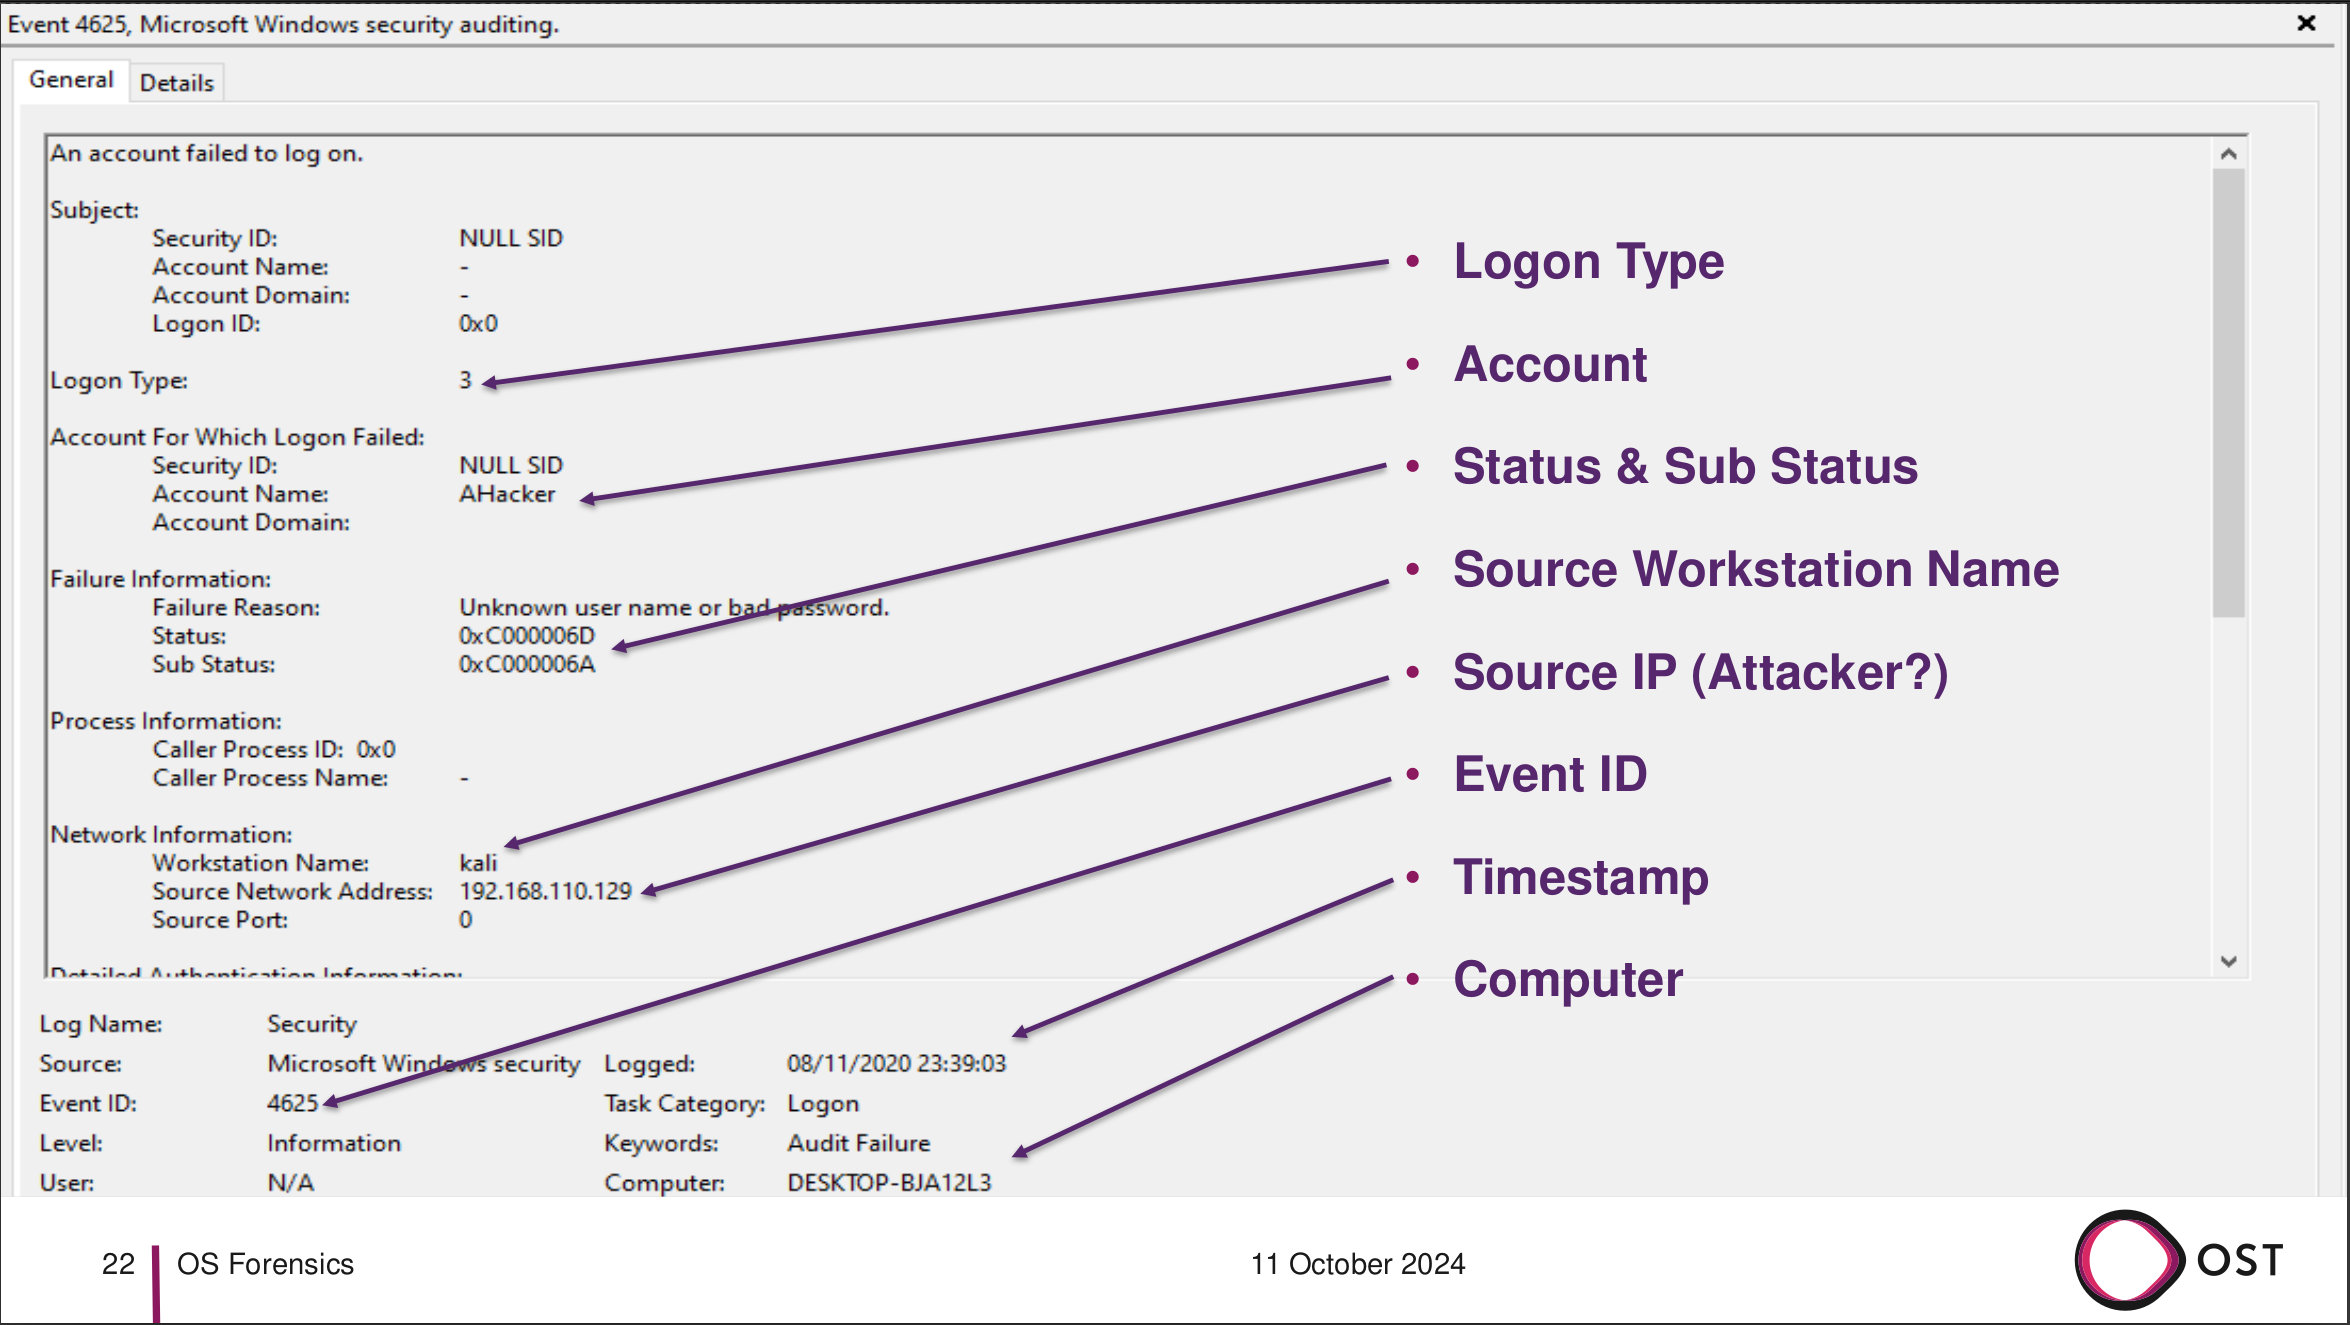
\includegraphics[width=\textwidth]{resources/05-event-example.png}
\end{center}

\subsubsection*{Command Line Auditing}
\begin{itemize}
   \item Process creation is not logged by default
   \begin{itemize}
       \item Enable in GPO
   \end{itemize}
   \item Results in:\\
   Event 4688 as "A new process has been created"
   \begin{itemize}
       \item 4688 will show any processes created by anybody including malware and attackers
   \end{itemize}
\end{itemize}

\textbf{Forensics Use}

\begin{itemize}
   \item User Account
   \item Parent process  
   \item Command line arguments
\end{itemize}

\subsubsection*{4648 Explicit Credential Logon}

"A user successfully logged on to a computer using explicit credentials while already logged on as a different user"

\begin{itemize}
   \item RunAs mostly
   \item Cobalt Strike spawnas or similar
   \item May indicate RDP (NLA use on source system)
   \item PsExec sometimes
\end{itemize}

\textbf{Check}
\begin{itemize}
   \item Account
   \item Target Server
   \item Process Information
\end{itemize}

\subsubsection*{4720 Account Creation}

\begin{itemize}
   \item Subject: Account authorizing the creation
   \item New Account: Information 
   \item Time the account was created
   \item Check for 4728 / 4732 / 4756 events (Member was added to a security-enabled group)
\end{itemize}

\textbf{When to expect?}

\begin{itemize}
   \item Uncommon
   \item Noisy (Easy to detect)
   \item May be a Pentest or Red Team making noise
\end{itemize}

\subsubsection*{Lateral Movement Example}
\begin{center}
  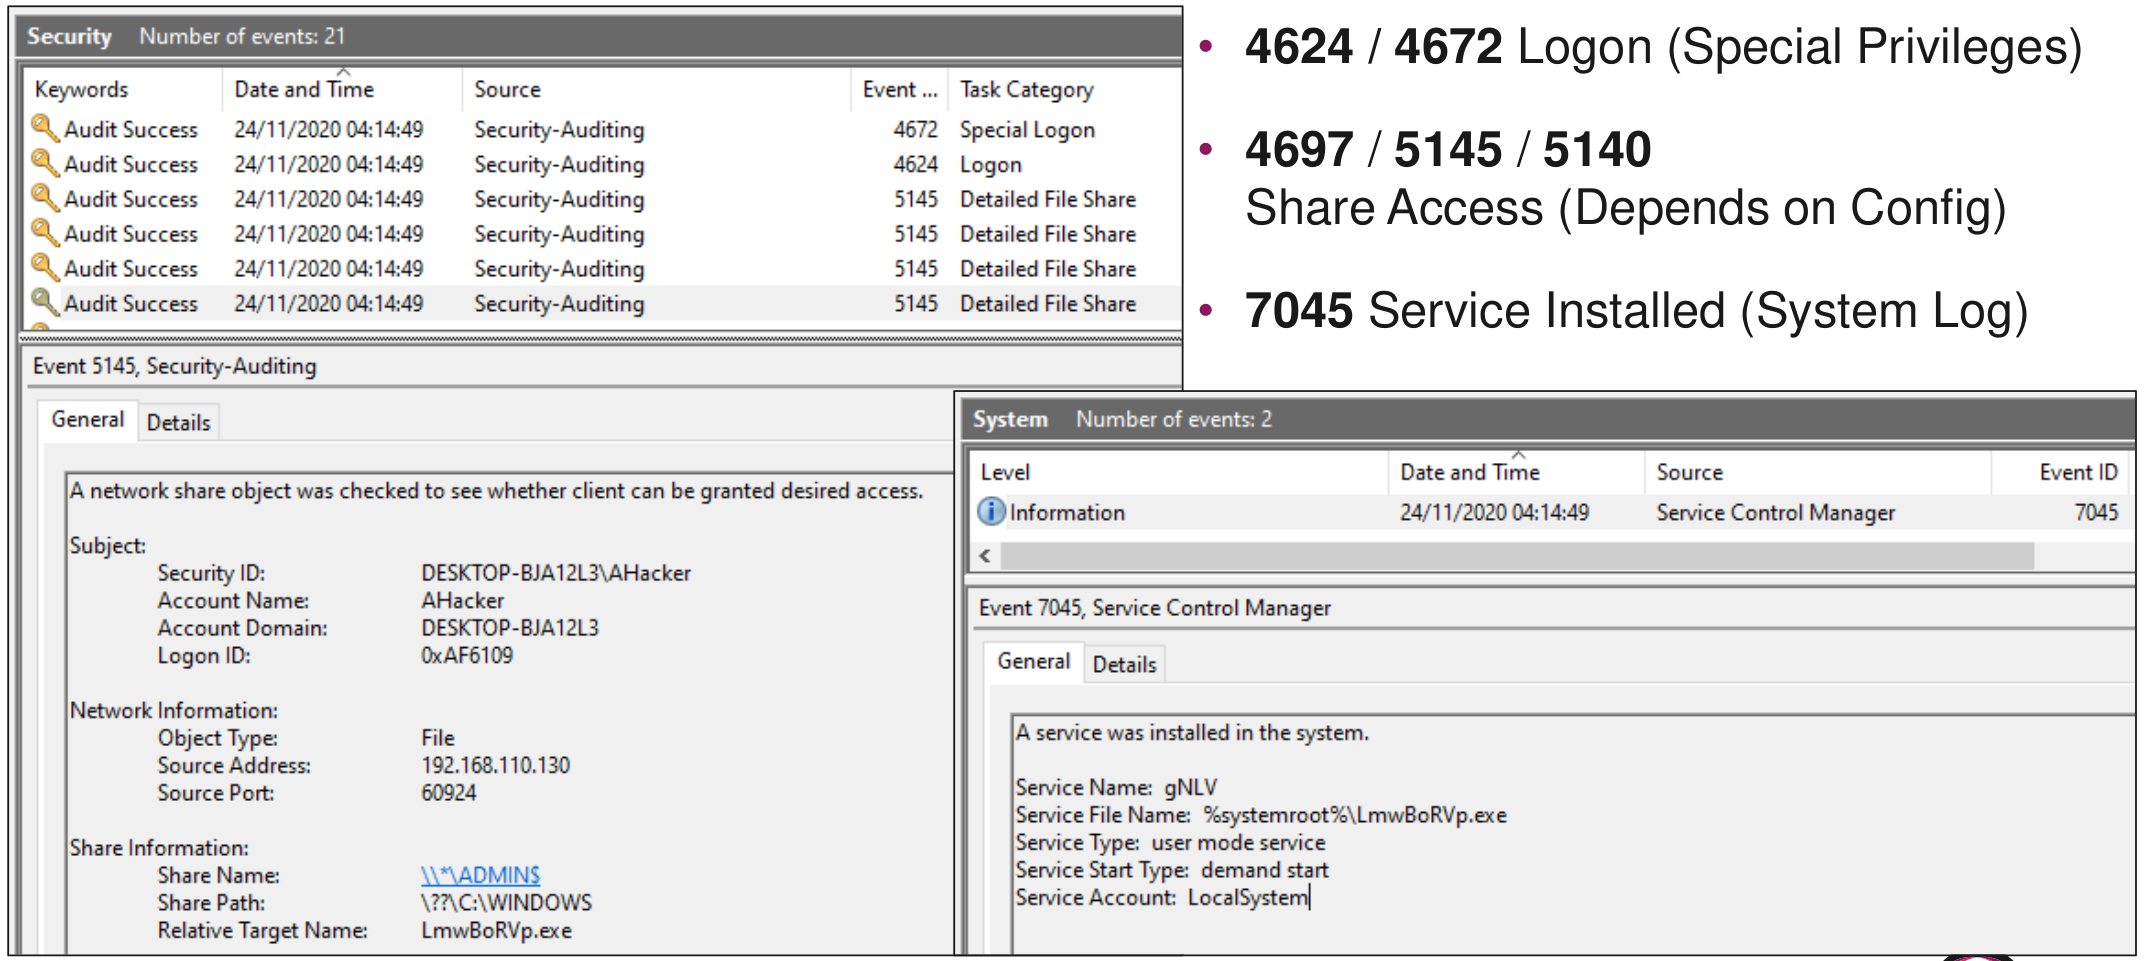
\includegraphics[width=\textwidth]{resources/05-lateral-movement.png}
\end{center}

\subsubsection*{Scheduled Tasks?}
\begin{itemize}
   \item 4698: A scheduled task was created
   \item 4700: A scheduled task was enabled
\end{itemize}

Look into Task Scheduler Event Log

\subsubsection*{PowerShell Event Logs}
PowerShell/Operational Log holds the most data
\begin{itemize}
    \item 4103 Module/Pipeline output logging
    \item 4104 Script block logging
    \begin{itemize}
        \item PowerShell Version 5+ has automatic logging of suspicious scripts\\
        $\rightarrow$ Records 4104 with a Warning Level
        \item Watch out for downgrade (powershell -Version 2 ...)
    \end{itemize}
    \item Often Obfuscated Payloads
\end{itemize}

PowerShell.evtx is older and may hold some data
\begin{center}
  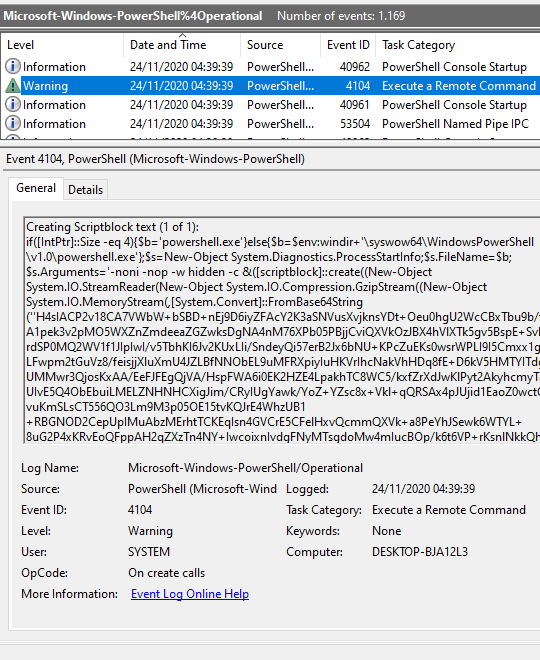
\includegraphics[scale=0.5]{resources/05-event-logs.png}
\end{center}

\subsubsection*{PowerShell.evtx}
\begin{itemize}
    \item EID 400 The engine status is changed from None to Available.
    \begin{itemize}
        \item This event indicates the start of a PowerShell activity, whether local or remote.
    \end{itemize}

    \item EID 600 Provider "XYZ" is Started.
    \begin{itemize}
        \item Indicates that providers such as WSMan start to perform a PowerShell activity on the system, for example, "Provider WSMan Is Started".
    \end{itemize}

    \item EID 403 The engine status is changed from Available to Stopped
    \begin{itemize}
        \item This event records the completion of a PowerShell activity.
    \end{itemize}

    \item HostName field in message details
    \begin{itemize}
        \item For a local activity: HostName = ConsoleHost
        \item Remote activity: HostName = ServerRemoteHost (on the system that is accessed)
    \end{itemize}
\end{itemize}

\subsubsection*{PowerShell Logging}

\paragraph*{PSReadline}
\begin{itemize}
    \item Records last 4096 typed commands
    \item Enabled by default (can be disabled)
    \item \verb|%appdata%\Microsoft\Windows\PowerShell\PSReadLine\ConsoleHost_history.txt|
\end{itemize}

\paragraph*{Transcript Logs}
\begin{itemize}
    \item Default: \verb|%userprofile%\Documents|
    \item Needs to be enabled (Start-Transcript / GPO)
    \item Logs PS input and output at the terminal
\end{itemize}

\subsubsection*{USB Devices}
Devices and their device drivers appear in the Device Manager MMC snap-in

\paragraph*{System.evtx}
\begin{itemize}
    \item 10000 DriverFramework-Usermode - driver package is being installed
    \item 10100 DriverFramework-Usermode - the driver package installation has succeeded
    \item 20001 User Plug-n-Play Device Event - Device Installation
\end{itemize}

\paragraph*{Microsoft-Windows-NTFS\%4Operational.evtx}
\begin{itemize}
    \item 142 - Free space on the drive and the volume name
\end{itemize}

\paragraph*{Microsoft-Windows-Partition\%4Diagnostic.evtx}
\begin{itemize}
    \item 1006
\end{itemize}

\subsection{Domain Controller Events}
\subsubsection{NTLM authentication}
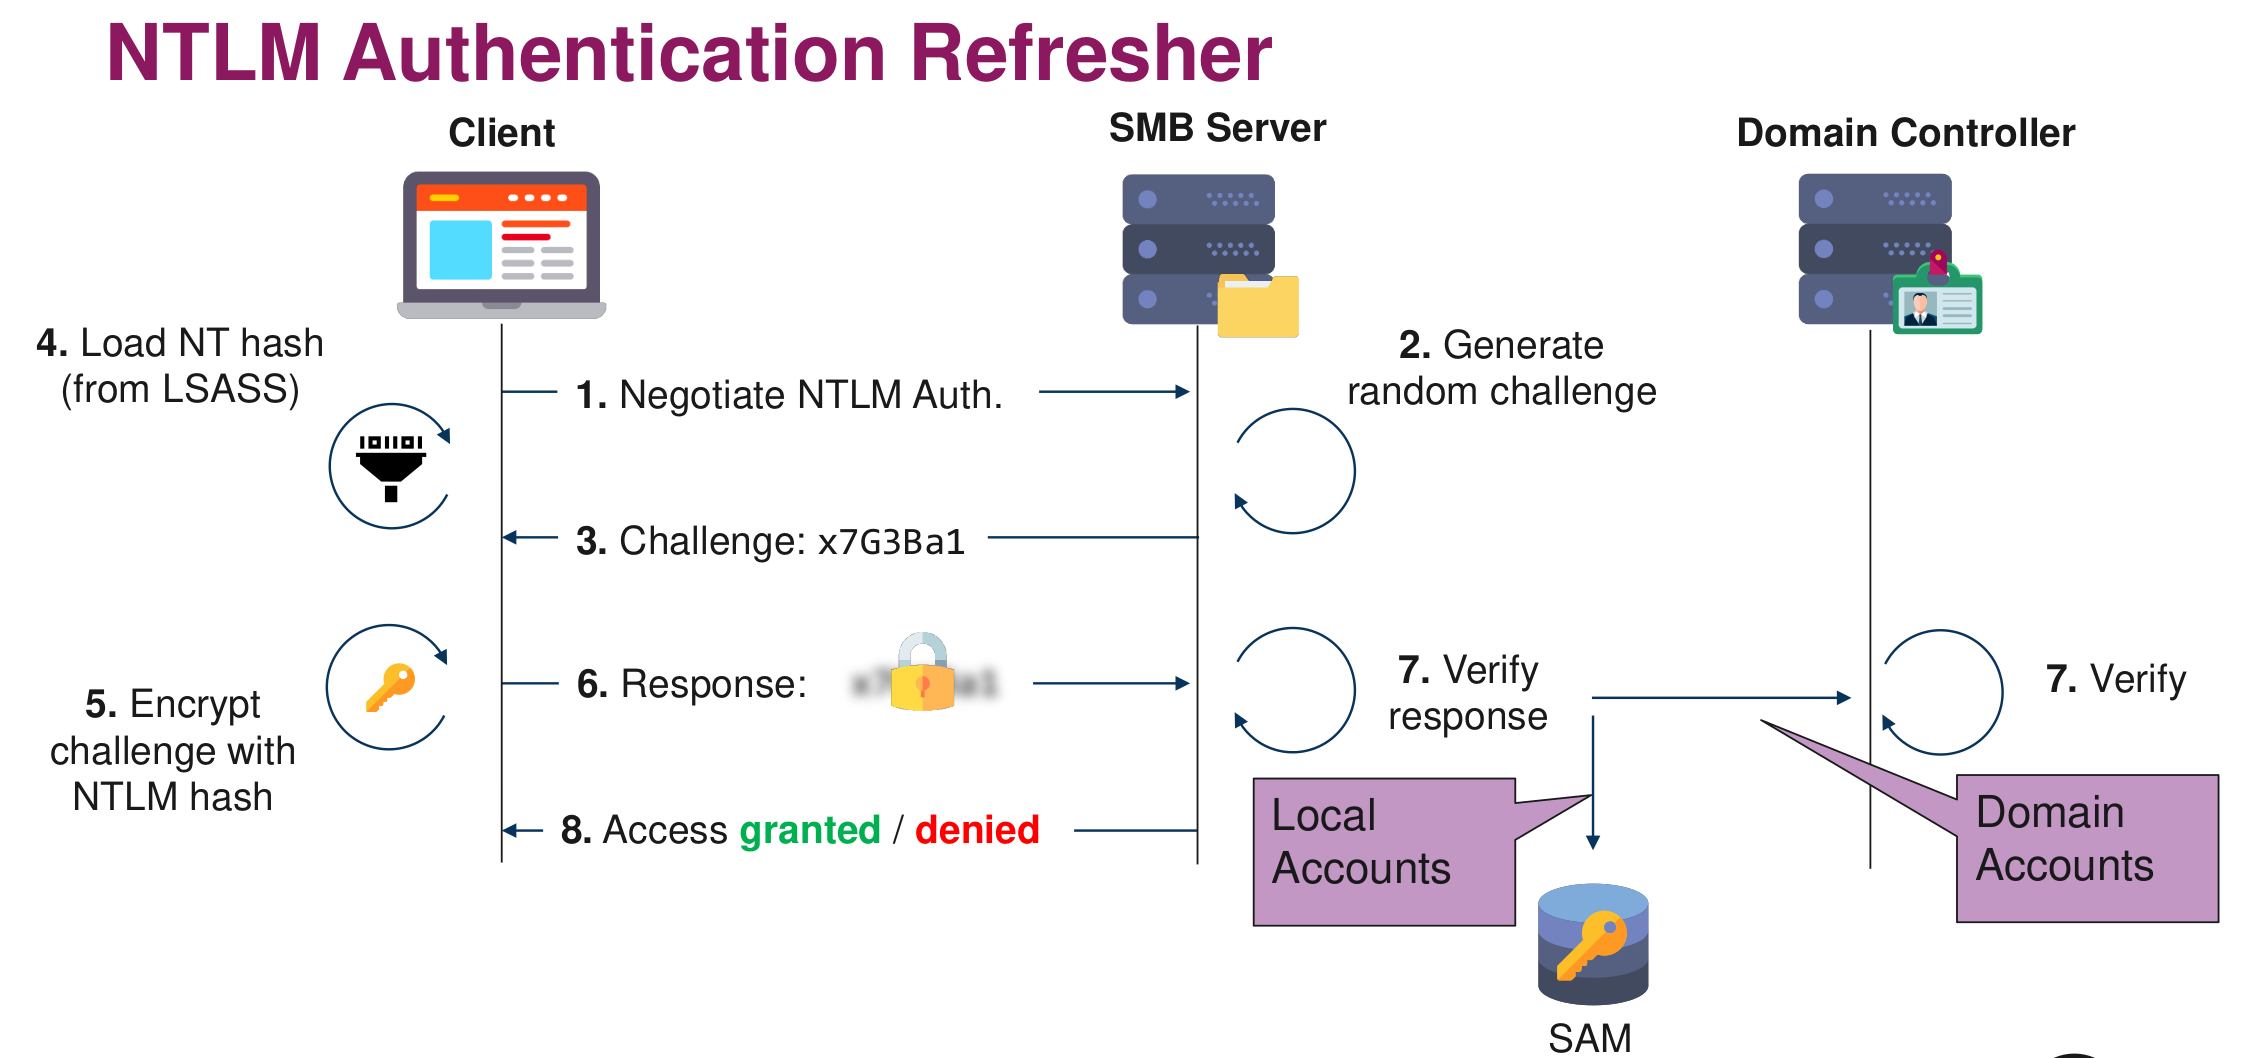
\includegraphics[width=\textwidth]{resources/05-ntlm-authentication.png}
\section*{NTLM Authentication Flow}
\begin{enumerate}
\item Client initiates NTLM authentication with SMB server
\item Server generates challenge
\item Server sends challenge ($x7G3Ba1$) to client
\item Client retrieves NT hash from LSASS
\item Client encrypts challenge using NT hash
\item Client sends encrypted response
\item Server verifies with local and domain accounts
\item Server grants/denies access
\end{enumerate}

\subsubsection{Kerberos authentication}
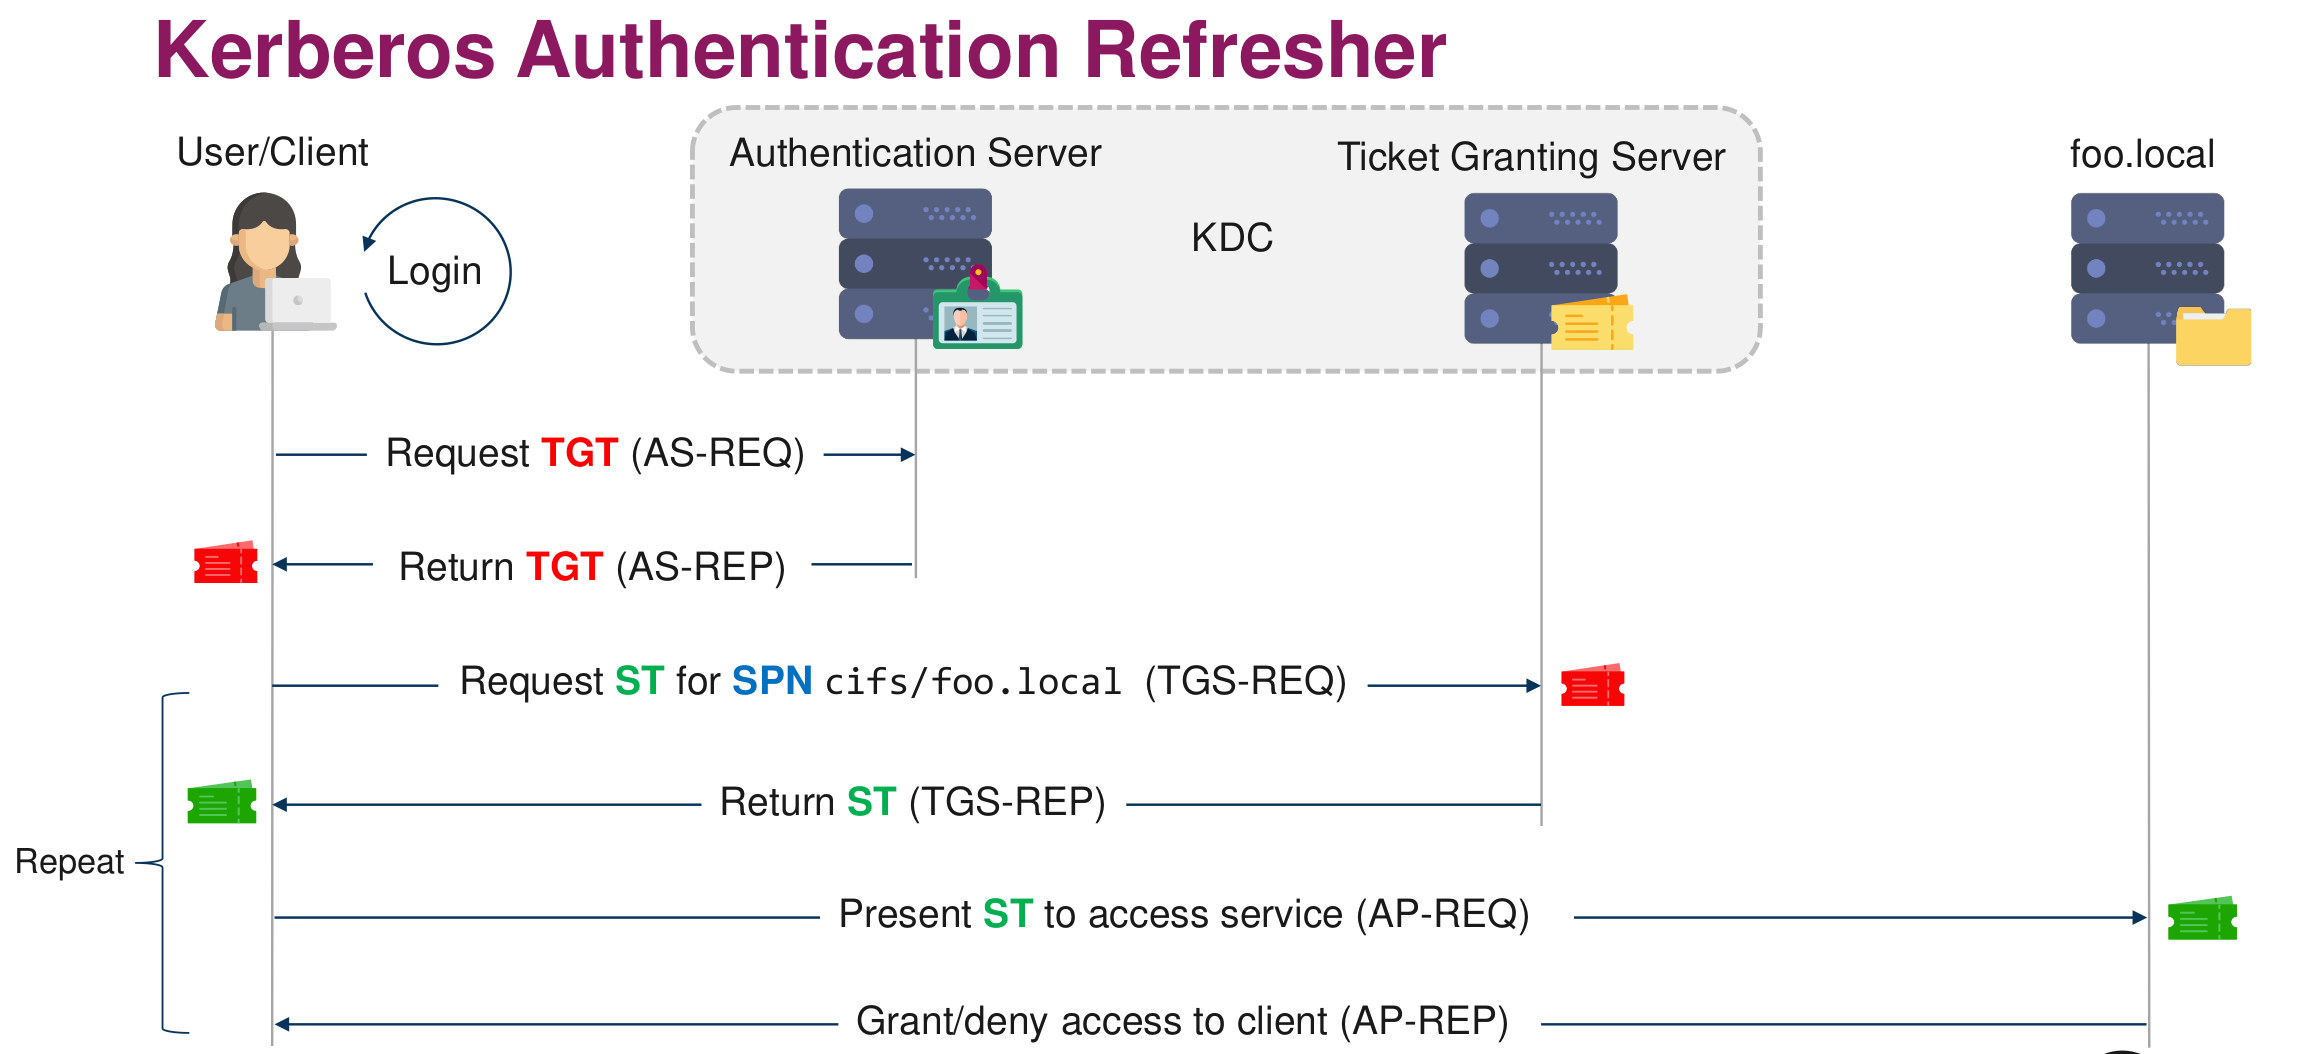
\includegraphics[width=\textwidth]{resources/05-kerberos-authentication.png}
\section*{Kerberos Authentication Flow}
\begin{enumerate}
\item Client requests TGT (AS-REQ) from Authentication Server/KDC
\item Authentication Server returns TGT (AS-REP)
\item Client requests ST for \texttt{cifs/foo.local} (TGS-REQ)
\item Ticket Granting Server returns ST (TGS-REP)
\item Client presents ST to service (AP-REQ)
\item Service grants/denies access (AP-REP)
\end{enumerate}

\subsection*{Account Logon Events (Domain Controller)}
\subsubsection*{Logged on the Authenticating System}
\textbf{Logged on the Authenticating System}
\begin{itemize}
    \item Domain Account → Logged on Domain Controller
    \item Local Account → Logged on Local System → Allows for good Hunting
\end{itemize}

\subsubsection*{Kerberos Authentication}
\begin{itemize}
    \item 4768: TGT was granted → Login success
    \item 4769: TGS requested → Service access successful 
    \item 4771: Pre-Authentication failed
\end{itemize}

\subsubsection*{NTLM Authentication}
\begin{itemize}
    \item 4776: Account Authentication (Success / Fail)
\end{itemize}

\begin{table}[h]
\begin{tabularx}{\textwidth}{|X|X|X|X|X|}
\hline
Event & Description &  Remote Host & Target & Payload Data2 \\
\hline
4776& NTLM authentication request & & lab\_admin &Workstation: Forensic \\
\hline
4776 & NTLM authentication request & & lab\_admin &Workstation: Forensic \\
\hline
4768 & A Kerberos authentication ticket (TGT) was requested &  ::ffff:10.0.1.10:58139 & \lstinline|winattacklab.local\\lab\_admin |& ServiceName: krbtgt \\
\hline
4769 & A Kerberos service ticket was requested & ::ffff:10.0.1.10:58140 & \lstinline|WINATTACKLAB.LOCAL\\lab\_admin| & \lstinline|ServiceName: CLIENT1$| \\
\hline
4769 & A Kerberos service ticket was requested & ::ffff:10.0.1.10:58146 & \lstinline|WINATTACKLAB.LOCAL\\lab\_admin| & ServiceName: krbtgt \\
\hline
4624 & Successful logon &- (10.0.1.10) & WINATTACKLAB.LOCAL\textbackslash{}lab\_admin| & LogonType 3 \\
\hline
4624 & Successful logon &- (10.0.1.10) & WINATTACKLAB.LOCAL\textbackslash{}CLIENT1\$ & LogonType 3 \\
\hline
\end{tabularx}
\end{table}

\subsection*{Kerberoasting}
\begin{itemize}
    \item Attacker is requesting RC4 encrypted Kerberos service tickets (TGS)
    \item Usually cracking the tickets offline
    \item 4769: A Kerberos service ticket (TGS) was requested
    \begin{itemize}
        \item Kerberos RC4 encrypted tickets have Ticket Encryption Type set to 0x17
    \end{itemize}
    \item Filter out requests from service accounts
    \item Filter on Audit Success
\end{itemize}


\subsection*{User Rights Enumeration}

\textbf{Process:} SharpHound enumerates local group membership by querying Windows SAM database via SAM-R protocol (port 445).

\textbf{Access Note:} All authenticated users can access SAMR on DCs and RODCs, though local SAM database on DCs is rarely used.

\textbf{BloodHound Edges:}
\begin{itemize}
    \item \texttt{AdminTo}: Local Administrators group members
    \item \texttt{CanRDP}: Remote Desktop Users group members  
    \item \texttt{CanPSRemote}: Distributed COM Users group members
    \item \texttt{ExecuteDCOM}: Remote Management Users group members
\end{itemize}

\subsection*{Detectable Default Events}
\begin{itemize}
    \item 4798: A user's local group membership was enumerated
    \item 4799: A security-enabled local group membership was enumerated
\end{itemize}

\subsection*{Forensics Readiness}
\begin{itemize}
    \item Detailed File Share Auditing
    \begin{itemize}
        \item Example: SYSVOL files storing rules: Audit Groups.xml and GptTmpl.inf access
    \end{itemize}
    \item Quite a lot of events
    \item 5145: Network share object access check
\end{itemize}

\begin{table}[h]
\begin{tabularx}{\textwidth}{|l|X|l|X|X|l|}
\hline
Event & Description & User & Remote Host / Target & Logon ID & Type \\
\hline
4624 & Successful logon & winattacklab\textbackslash{}aalfort & - (10.0.1.10) & LogonId: 0x59BBCD & 3 \\
\hline
4799 & A security-enabled local group membership was enumerated & winattacklab\textbackslash{}aalfort & Target: Builtin\textbackslash{}Administrators (S-1-5-32-544) & SubjectLogonId: 0x59BBCD & \\
\hline
4799 & A security-enabled local group membership was enumerated & winattacklab\textbackslash{}aalfort & Target: Builtin\textbackslash{}Distributed COM Users (S-1-5-32-562) & SubjectLogonId: 0x59BBCD & \\
\hline
4799 & A security-enabled local group membership was enumerated & winattacklab\textbackslash{}aalfort & Target: Builtin\textbackslash{}Remote Management Users (S-1-5-32-580) & SubjectLogonId: 0x59BBCD & \\
\hline
4799 & A security-enabled local group membership was enumerated & winattacklab\textbackslash{}aalfort & Target: Builtin\textbackslash{}Remtoe Desktop Users (S-1-5-32-555) & SubjectLogonId: 0x59BBCD & \\
\hline
\end{tabularx}
\end{table}

\subsection{Automated Analysis Tools}

\begin{itemize}
\item Simple Event Log Analysis Tools (No ELK/Splunk required):

\item \textbf{DeepBlueCLI} \href{https://github.com/sans-blue-team/DeepBlueCLI}{github.com/sans-blue-team/DeepBlueCLI}
    \begin{itemize}
        \item Basic regex search and hunting (outdated)
    \end{itemize}

\item \textbf{Chainsaw} \href{https://github.com/WithSecureLabs/chainsaw}{github.com/WithSecureLabs/chainsaw}
    \begin{itemize}
        \item String/Event ID search
        \item Custom + Sigma rule processing
        \item ShimCache/SRUM analysis
    \end{itemize}

\item \textbf{APT-Hunter} \href{https://github.com/ahmedkhlief/APT-Hunter}{github.com/ahmedkhlief/APT-Hunter}

\item \textbf{Events-Ripper} \href{https://github.com/keydet89/Events-Ripper}{github.com/keydet89/Events-Ripper}

\item \textbf{Hayabusa} \href{https://github.com/Yamato-Security/hayabusa}{github.com/Yamato-Security/hayabusa}
\end{itemize}

\subsubsection*{Hayabusa}
Windows event log fast forensics timeline generator and threat hunting tool

\begin{itemize}
\item Detects known bad behavior in Event Logs
    \begin{itemize}
        \item 2400 Sigma rules + 130+ built-in detection rules
    \end{itemize}
    
\item Can be run:
    \begin{itemize}
        \item On single systems (live analysis)
        \item By gathering logs from multiple systems (offline)
        \item Via Velociraptor artifact
    \end{itemize}

\item Outputs CSV
\end{itemize}

\begin{verbatim}
.\hayabusa-1.4.1-win-x64.exe -f eventlog.evtx
.\hayabusa-1.4.1-win-x64.exe -d .\hayabusa-sample-evtx
.\hayabusa-1.4.1-win-x64.exe -d .\hayabusa-sample-evtx -r .\rules\hayabusa.default -o results.csv
\end{verbatim}

\section{exercise}



